\documentclass[14pt,a4paper]{report}  %紙張設定
\usepackage{xeCJK}%中文字體模組
\setCJKmainfont{標楷體} %中文字體
\usepackage{amsmath,amssymb}%數學公式、符號
\usepackage{graphicx, subfig}%圖形
\usepackage{graphicx, subfig}%圖片模組
\usepackage{type1cm} %調整字體絕對大小
\usepackage{textpos} %設定文字絕對位置
\usepackage[top=2.5truecm,bottom=2.5truecm,
left=3truecm,right=2.5truecm]{geometry}
\usepackage{titlesec} %目錄標題設定模組
\usepackage{titletoc} %目錄內容設定模組
\usepackage{caption} %圖片標題設定
\usepackage{CJK} %中文模組
\usepackage{CJKnumb} %中文數字模組
%\usepackage{wallpaper} %浮水印
\usepackage{float}
\usepackage{enumerate}
\renewcommand{\baselinestretch}{1.0} %設定行距1.0

\newcommand{\thirty}{\fontsize{30pt}\baselineskip\selectfont}%字體大小30pt
\newcommand{\twentyfour}{\fontsize{24pt}{\baselineskip}\selectfont}%字體大小24pt
\newcommand{\twenty}{\fontsize{20pt}{\baselineskip}\selectfont}%字體大小20pt
\newcommand{\eigh}{\fontsize{18pt}{\baselineskip}\selectfont}%字體大小18pt
\newcommand{\sixteen}{\fontsize{16pt}{\baselineskip}\selectfont}%字體大小16pt
\newcommand{\fourteen}{\fontsize{14pt}{\baselineskip}\selectfont}%字體大小14pt
\newcommand{\twelve}{\fontsize{12pt}{\baselineskip}\selectfont}%字體大小12pt

%設定章節標題內容
\titleformat{\chapter}[hang]{\center \twenty \bf}{\twenty 第\CJKnumber{\thechapter}章}{1em}{}[]
\titleformat{\section}[hang]{\raggedright \eigh \bf}{\eigh 第{\thesection}節}{1em}{}[]
\titleformat{\subsection}[hang]{\raggedright \sixteen \bf}{\sixteen {\thesubsection}}{1em}{}[]
%章節間距
\titlespacing*{\chapter} {0pt}{0pt}{18pt}
\titlespacing*{\section} {0pt}{12pt}{6pt}
\titlespacing*{\subsection} {0pt}{6pt}{6pt}
%設定目錄內容
\titlecontents{chapter}[11mm]{}{\normalfont\fontsize{14pt}{2.5pt}\bfseries\makebox[3.5em][l]
{第\CJKnumber{\thecontentslabel}章}}{}{\titlerule*[0.7pc]{.}\contentspage}
\titlecontents{section}[18mm]{}{\fourteen \makebox[2em][l]
{\fourteen \thecontentslabel}}{}{\titlerule*[0.7pc]{.}\contentspage}
\titlecontents{subsection}[25mm]{}{\fourteen \makebox[2.5em][l]{{\fourteen \thecontentslabel}}}{}{\titlerule*[0.7pc]{.}\contentspage}
%設定圖表目錄內容
\newcommand{\loflabel}{圖}
\newcommand{\lotlabel}{表}
\captionsetup{font={Large}} %設定標題大小
\captionsetup[figure]{name=圖} %固定標題名稱

\begin{document}
    {\renewcommand\baselinestretch{1.4}\selectfont %設定以下行距
    {\begin{center} %以下文字置中
        \twentyfour{國立虎尾科技大學}\\{機械設計工程系}\\{專題製作報告}\\
        \hspace*{\fill} \\
        \bf \thirty {Pyslvs-UI 平面多連桿機構套件之合成與應用}\\
        {\renewcommand\baselinestretch{1.3}\selectfont %設定以下行距
        \bf \thirty {Synthesis and Application of Pyslvs-UI Planar Multi-link Mechanism Package}\\}
    \end{center}}
    \par} %結束指定行距

     {\renewcommand\baselinestretch{1.2}\selectfont %設定以下行距
    {\begin{textblock}{30}(1.45,1.1) %{寬度}(以左上角為原點之右移量,下移量)
    \noindent \eigh \makebox[6em][s]{指導教授}\enspace:\qquad
    \eigh \makebox[8em][s]{李武鉦}\\ %\noindent指定首行不進行縮排
    \eigh \makebox[6em][s]{班級}\enspace:\qquad
    \eigh \makebox[8em][s]{四設計三甲} \\ %\makebox為文本盒子
    \eigh \makebox[6em][s]{學生}\enspace:\qquad
    {\begin{minipage}[t][9.8em][s]{12em}
    \eigh \setlength{\baselineskip}{10pt plus 2pt}
    林昱秀\qquad40723102\vfill 林晏瑩\qquad40723103\vfill 劉光智\qquad40723145\vfill 吳佳穎\qquad40723153\vfill 蔡育灃\qquad40723245
    \end{minipage}}
    \end{textblock}} %指定以下文字整體偏移至頁面的絕對位置
    \par} %結束指定行距

    {\begin{textblock}{12}(0,6.8)
    {\begin{center}
    \noindent \eigh \makebox[12em][s]{中華民國一一零年四月}
    \end{center}}
    \end{textblock}}
    \newpage
%專題製作合可證明
 {\renewcommand\baselinestretch{1.4}\selectfont %設定以下行距
 {\begin{center}
    {\eigh {國立虎尾科技大學 \qquad 機械設計工程系}\\{學生專題製作合格認可證明}\\
    \hspace*{\fill} \\ %似enter鍵換行
    \par}
     \end{center}}
    {\begin{textblock}{60}(1.85,0.8)
    \noindent \fourteen 專題製作修習學生\enspace:\quad
    {\begin{minipage}[t]{10em}\underline{四設三甲\enspace 40723102\enspace 林昱秀}\\ \underline{四設三甲\enspace 40723103\enspace 林晏瑩}\\ \underline{四設三甲\enspace 40723145\enspace 劉光智}\\ \underline{四設三甲\enspace 40723153\enspace 吳佳穎}\\ \underline{四設三乙\enspace 40723245\enspace 蔡育灃}\\ %下劃線符號指令
    \end{minipage}}
         \par} %結束指定行距
    {\renewcommand\baselinestretch{1.2}\selectfont %設定以下行距
    {\begin{textblock}{30}(1.8,4)
    \noindent \fourteen 專題製作題目\enspace :\quad Pyslvs-UI 平面多連桿機構套件之合成與應用
    \hspace*{\fill} \\
    \hspace*{\fill} \\
    \noindent \fourteen 經評量合格,特此證明
    \hspace*{\fill} \\
    \hspace*{\fill} \\
    \noindent \fourteen \makebox[6em][s]{評審委員}\enspace:\quad
    {\begin{minipage}[t]{6em} \underline{            }\\ \underline{            }\\ \underline{            }\\
    \end{minipage}}
    \end{textblock}}
    {\begin{textblock}{10}(1.8,9)
    {\begin{flushleft}
    \fourteen \makebox[6em][s]{指導老師}\enspace:\quad \underline{            }\\
    \fourteen \makebox[6em][s]{系主任}\enspace:\quad \underline{            }\\
    \hspace*{\fill} \\
    \fourteen \makebox[12em][s]{中華民國一一零年}
    \fourteen \makebox[9em][s]{四月二十九日}
    \end{flushleft}}
    \end{textblock}}
    \end{textblock}}
     \par} %結束指定行距
     \newpage
%摘要
	\pagenumbering{roman} %設定以下頁碼為羅馬數字
    \addcontentsline{toc}{chapter}{\fourteen{摘要}} %將摘要加入目錄
    \begin{center}
	\twenty \bf{摘要}\\
	\end{center}
	\begin{flushleft}
	\fourteen
	{生產自動化是現今工業界中最重要的一環,如何以更低的成本與縮短生產製程,		來提高在國際上的競爭力,是大家所努力的目標,而身為未來二十一世紀的一員,		更需了解其重要性。}
    \end{flushleft}
	\begin{center}
	\fontsize{14pt}{2.5pt}{關鍵字:機構模擬、機構分析}
	\end{center}
%目錄
\addcontentsline{toc}{chapter}{\fourteen{目錄}} %將目錄加入目錄
{\begin{center}
\renewcommand{\contentsname}{\centerline{\fontsize{20pt}{\baselineskip}\selectfont\textbf{目\quad 錄}}}
{\fourteen \tableofcontents}
%圖表目錄
\addcontentsline{toc}{chapter}{\fourteen{圖表目錄}} %將圖表目錄加入目錄
\renewcommand{\listfigurename}{\centerline{\fontsize{20pt}{\baselineskip}\selectfont\textbf{圖\quad 表\quad 目\quad 錄 }}}
\renewcommand{\numberline}[1]{\loflabel~#1\hspace*{1em}}
{\fourteen \listoffigures}
\end{center}}
         
{\begin{center}
     \chapter{簡介}
     \end{center}}
     \pagenumbering{arabic} %設定以下頁碼為阿拉伯數字
     {\begin{flushleft}
        \fourteen{生產自動化是現今工業界中最重要的一環,如何以更低的成本與			縮短生產製程,來提高在國際上的競爭力,是大家所努力的目標,而身為未來			二十一世紀的一員,更需了解其重要性。
        \hspace*{\fill} \\
        目前於市面上的數位控制加工機(CNC),其成本昂貴,且體積龐大,故本組			決定運用在校所學之相關課程,以完成一部具有高精度、體積小與低成本(十			五萬元以下)的 PC-Based 三軸運動控制實驗台為研究目標,達成在教學上			的需要,並增加系內的實驗設備。
        \hspace*{\fill} \\
        本專題主要目的在了解伺服馬達的控制原理、三軸運動控制卡的使用方式、人			機介面程式的撰寫與增加機械實務加工的能力。
        }
        \end{flushleft}
        \newpage
      \section{研究背景與動機}
      \fourteen {隨著科技越來越發達網路上有許多機構分析的套件,但是鮮少有機構合成功能的套件,且大多為收費或無公開原始碼。而本專題所使用的套件-Pyslvs-UI為本研究室所開發的套件且有公開原始碼,因此此專題利用該套件來合成一登山車避震機構。}
      \section{研究目的}
      \section{研究方法}
      \fourteen {首先建立一現有登山車避震機構,再針對不影響現有自行車車架的尺寸但對於避震能力有較大影響的接頭利用遺傳演算法求解最佳位置以得到最佳連桿尺寸,接著將上述所得到的接頭位置和連桿長度利用Inventor自動產生對應連桿尺寸,後續利用xml格式匯入CoppeliaSim並利用CoppeliaSim API設定馬達讓該機構以一自由度進行運動模擬。上述流程如圖XXXX所示。}

    {\begin{center}
        \chapter{文獻探討}
        \end{center}}
      \section{平面機構分析套件}
      \section{平面機構合成套件}
      \subsection{MeKin2D}
       \hspace*{\fill} \\
       \fourteen {MeKin2D為一種用Free Pascal編寫的子程序包。主要功能使用模組化設計對平面連桿進行運動學模擬、盤式凸輪機構的合成與分析,如圖2.1、圖2.2。其中,MeKin2D的套件包含4個子程式。 分別有:}
       \begin{enumerate} 
       \item LibMec2D:定義偏移點將復雜形狀附加到運動的鏈接			上,並添加模擬線性和角度量度,作為向量的速度和加速度			以及運動點的軌跡
       \item LibMecIn:定義基本輸入,例如曲柄或滑塊
       \item LibAssur:對被動模塊進行建模
       \item LibCams:用於運動學合成並分析盤式凸輪
       \end{enumerate}
       \begin{figure}[H]
        \centering
        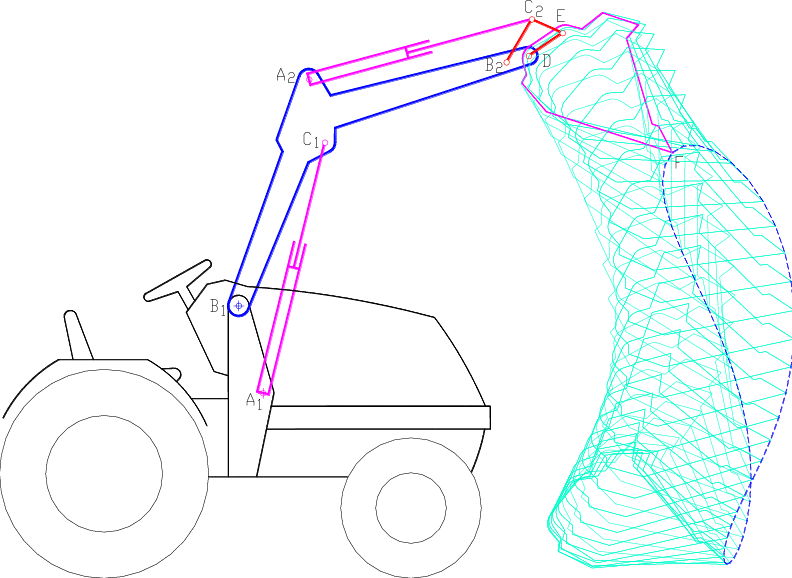
\includegraphics[scale=0.4]{平面連桿之運動學模擬.png} 
        \caption{平面連桿之運動學模擬} 
        \label{fig:scale}
        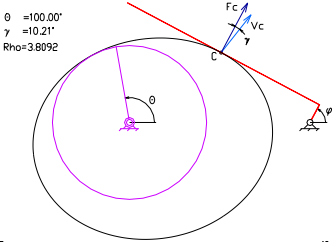
\includegraphics[scale=0.8]{盤式凸輪機構之合成與分析.png} 
        \caption{盤式凸輪機構之合成與分析} 
        \label{fig:scale}   
    	\end{figure}
    	 \hspace*{\fill} \\
       \subsection{MechDev}
       \hspace*{\fill} \\        
        \fourteen {MechDev是一種機構設計軟件,專注於可用性和機構設計功能。
基本功能為分析機構運動學、運動靜力學、帶有滾輪從動件或平面從動件的凸輪機構的合成與分析
}
	  \hspace*{\fill} \\
       \subsection{WinMecC}
       \hspace*{\fill} \\        
        \fourteen {WinMecC為一種計算機軟件,用於平面機構具有一個自由度和任意數量鏈接。基本功能為將機構的運動學和動力學分析所獲得的大量結果,顯示成數值化或圖視化、可以優化分析創建的任何機構,並依據特定點所期望遵循之路徑,進行機構合成。

}
      \newpage
      \section{自行車避震機構研究}
       \subsection{Single-pivot suspension(單軸懸架)}
       \hspace*{\fill} \\
       \fourteen {最簡單的懸架設計為單樞軸,使用搖臂連接後軸、主樞軸、避震器,特點在於後軸直接連接至主樞軸,避震器連接到搖臂上,搖桿環繞在主樞軸中心旋轉,槓桿比由避震器的位置決定,固定中心可在行駛過程預測懸架特性,但也意味著不同階段修改懸架特性能力有限,示意圖產品型號為 Orange Stage的 STAGE 6 FACTORY,如圖(2.1)。}
     \begin{figure}[H]
        \centering
        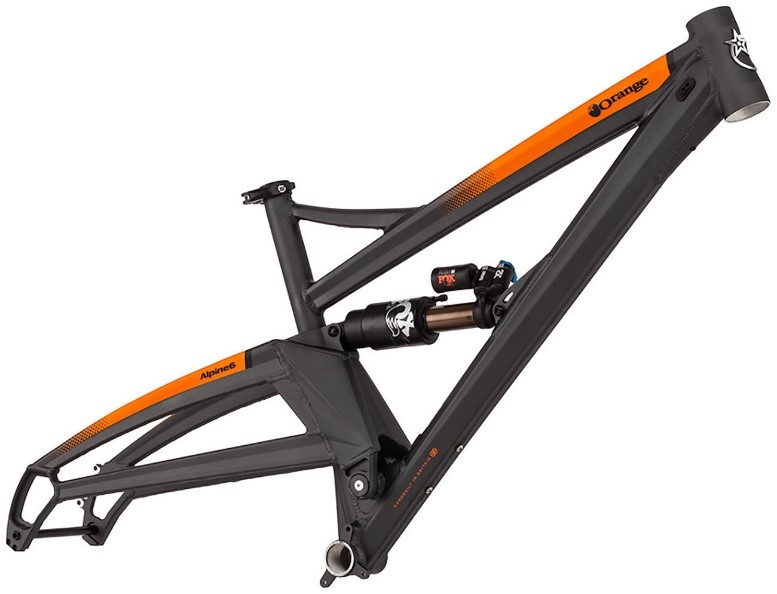
\includegraphics[scale=0.8]{單軸懸架.jpg} 
        %照片須放在和文檔相同之資料夾內
        \caption{單軸懸架} %有caption的圖才會編入目錄中
        \label{fig:scale} %此處的label相當於一個圖片的專屬標誌,目的是方便上下文的引用
    \end{figure}
       \hspace*{\fill} \\
       \subsection{Linkage-driven Single-pivot Suspension(連桿驅動之單樞軸懸架)}
       \hspace*{\fill} \\        
        \fourteen {如同單樞軸設計藉由後軸通過搖臂連接到主樞軸,增加聯動裝置在避震與搖臂間允許調整槓桿比率曲線,並在搖臂與避震器間建立連桿以改變槓桿比,搖臂圍繞在主軸旋轉且將中心固定於整個行程中,示意圖產品車架為Orange Stage的Orange 2020 Alpine 6 Frame 27.5,如圖(2.2)。}
     \begin{figure}[H]
        \centering
        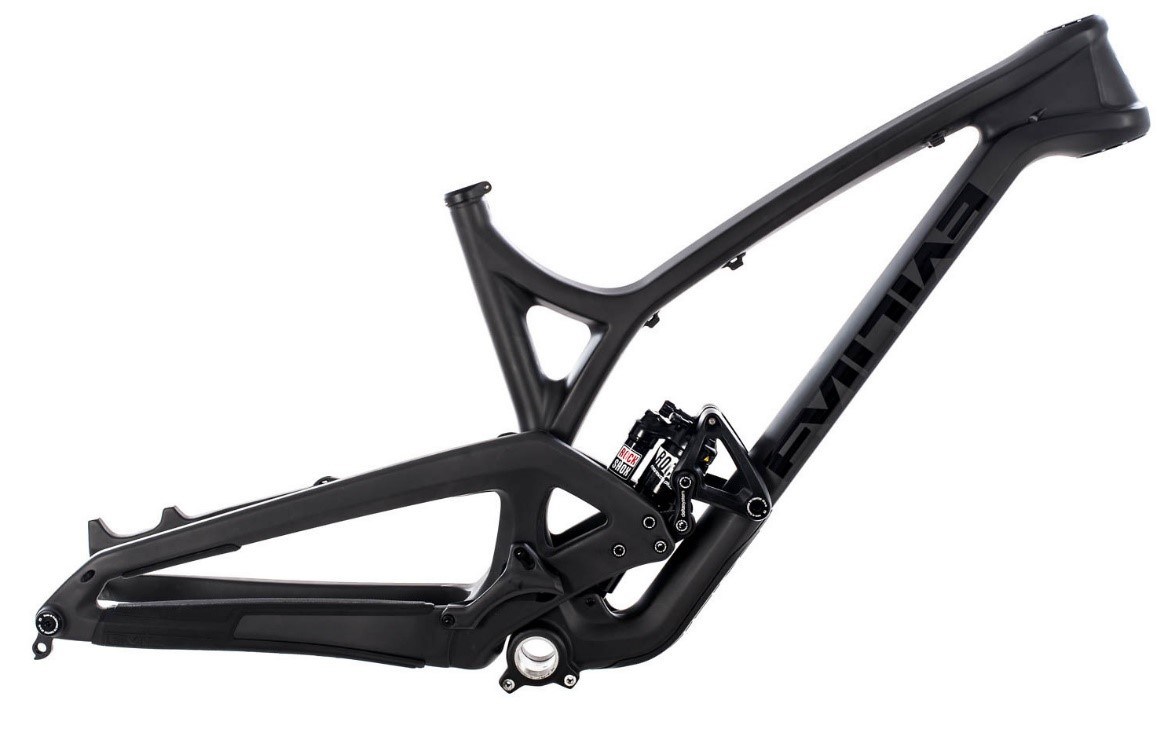
\includegraphics[scale=0.65]{連桿驅動之單樞軸懸架.jpg} 
        %照片須放在和文檔相同之資料夾內
        \caption{連桿驅動之單樞軸懸架} %有caption的圖才會編入目錄中
        \label{fig:scale} %此處的label相當於一個圖片的專屬標誌,目的是方便上下文的引用
    \end{figure}
        \newpage
        \subsection{High-Pivot Idler Suspension(高樞轉惰輪懸架)}
        \hspace*{\fill} \\
        \fourteen{通常建構在單樞軸或鏈接驅動的單樞軸設計上,其樞軸位置位於鏈條上方,為使控制鏈條增長,鏈輪惰輪將鏈條從鏈輪佈置到主樞軸的頂部或非常靠近主樞軸的位置,主樞軸定位在鏈輪上方更高的位置,使用單樞軸同時中心在整個行程中是固定的。
         \hspace*{\fill} \\  
但是,在撞擊過程中,後搖臂在主樞軸下方以曲線向上和向後旋轉,而不是在低樞軸位置向上和向後旋轉,且後軸路徑可以幫助懸架在方形撞擊中保持平穩。
		 \hspace*{\fill} \\  
鏈條繞到惰輪上,使鏈條與樞軸和後軸成一直線,大大減少了鏈增長的影響。惰輪的位置可以由設計人員用來增加或減少防下蹲的水平,但不會改變通常較高的防起落高度,如圖(2.3),產品來源為Forbidden Druid的Druid Frame – 2021。}
     \begin{figure}[hbt!]
        \centering
        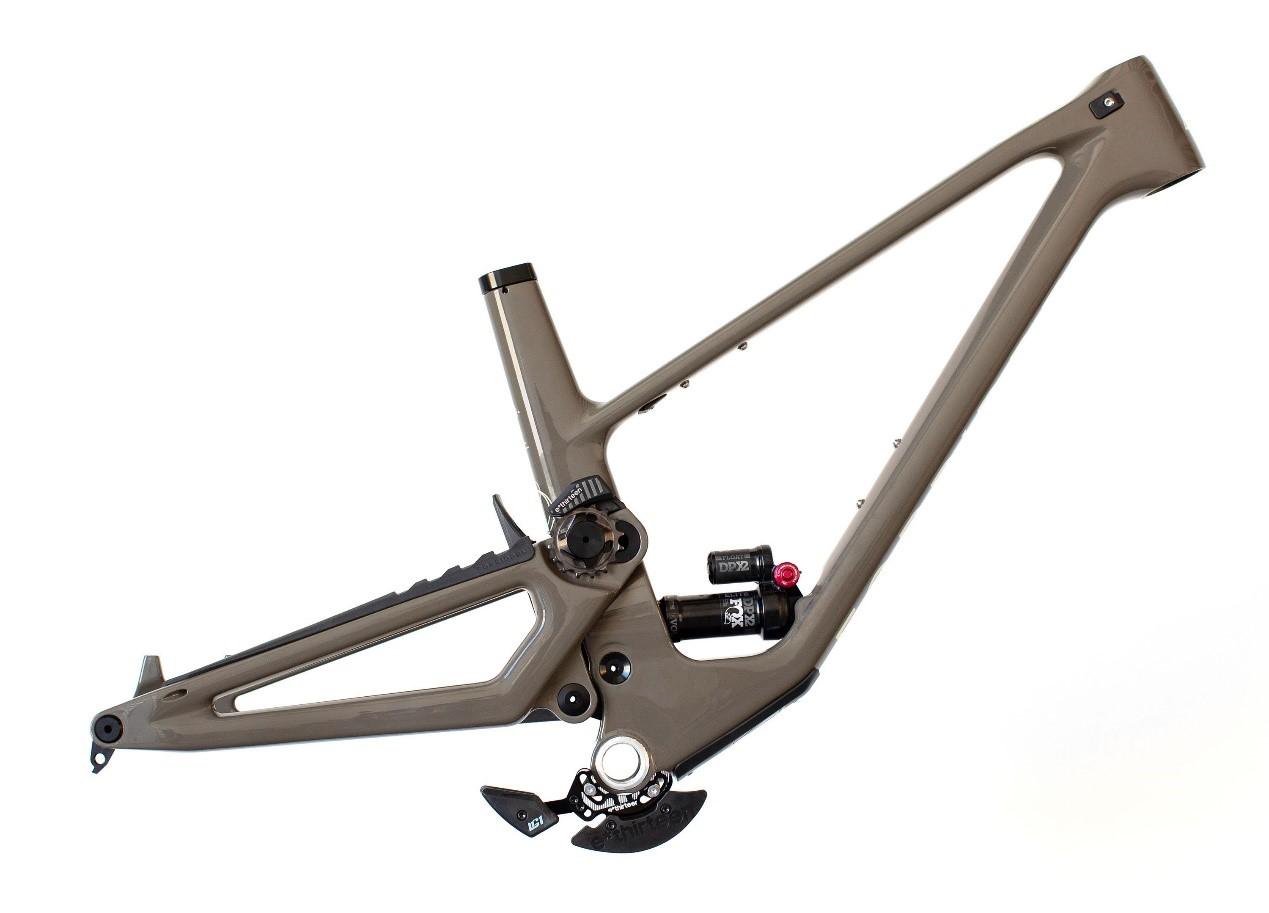
\includegraphics[scale=0.6]{高樞轉惰輪懸架.jpg} 
        %照片須放在和文檔相同之資料夾內
        \caption{高樞轉惰輪懸架} %有caption的圖才會編入目錄中
        \label{fig:scale} %此處的label相當於一個圖片的專屬標誌,目的是方便上下文的引用
    \end{figure}  
       \hspace*{\fill} \\
        \subsection{Twin-link Suspension(雙連桿懸掛)}
        \hspace*{\fill} \\
         \fourteen {搖臂通過兩個搖桿連桿安裝在框架上,從而將搖臂連接到主機樞軸,通過擺臂或搖臂連桿之一來驅動衝擊。
         \hspace*{\fill} \\  
         雙連桿懸架將樞軸的數量從一增加到四個,可修改中心位置,進而改變行程不同點的懸架特性,參考產品為Ibis’ DW-link Suspension的Mojo HD5 Frame – 2020,如圖(2.4)。}
     \begin{figure}[hbt!]
        \centering
        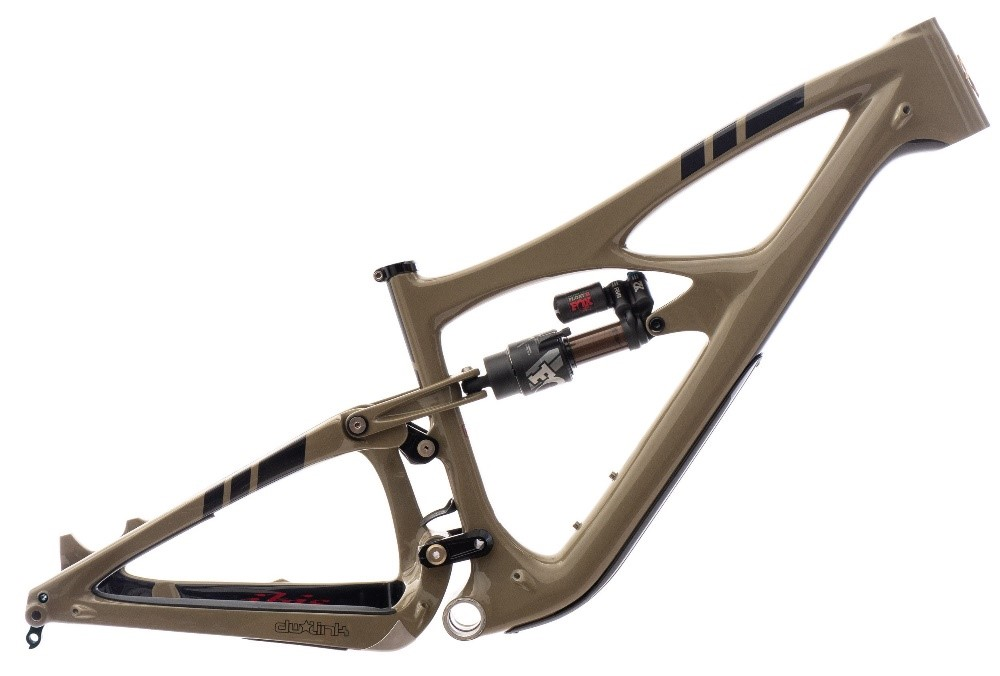
\includegraphics[scale=0.7]{雙連桿懸掛.jpg} 
        %照片須放在和文檔相同之資料夾內
        \caption{雙連桿懸掛} %有caption的圖才會編入目錄中
        \label{fig:scale} %此處的label相當於一個圖片的專屬標誌,目的是方便上下文的引用
    \end{figure}
    \newpage  
    	\hspace*{\fill} \\
        \subsection{Horst-link Suspension(霍斯特鏈懸掛)}
        \hspace*{\fill} \\
         \fourteen {特性在於樞軸底端的鏈條,後軸則安裝在腳撐上增加了樞軸,其修改後的軸距繞即時中心旋轉,改變行進路線的位置,可在行進的不同階段優化防下蹲與上抬。
         \hspace*{\fill} \\  
雙連桿懸掛相比,霍斯特連桿系統的較長連桿通常會提供更平滑的曲線,產品支架為RAAW Madonna的MADONNA V1 - FAST AND PREDICTABLE,如圖(2.5),產品為 Canyon Spectral的Izzo Pro Race 29,如圖(2.6)。}
     \begin{figure}[hbt!]
        \centering
        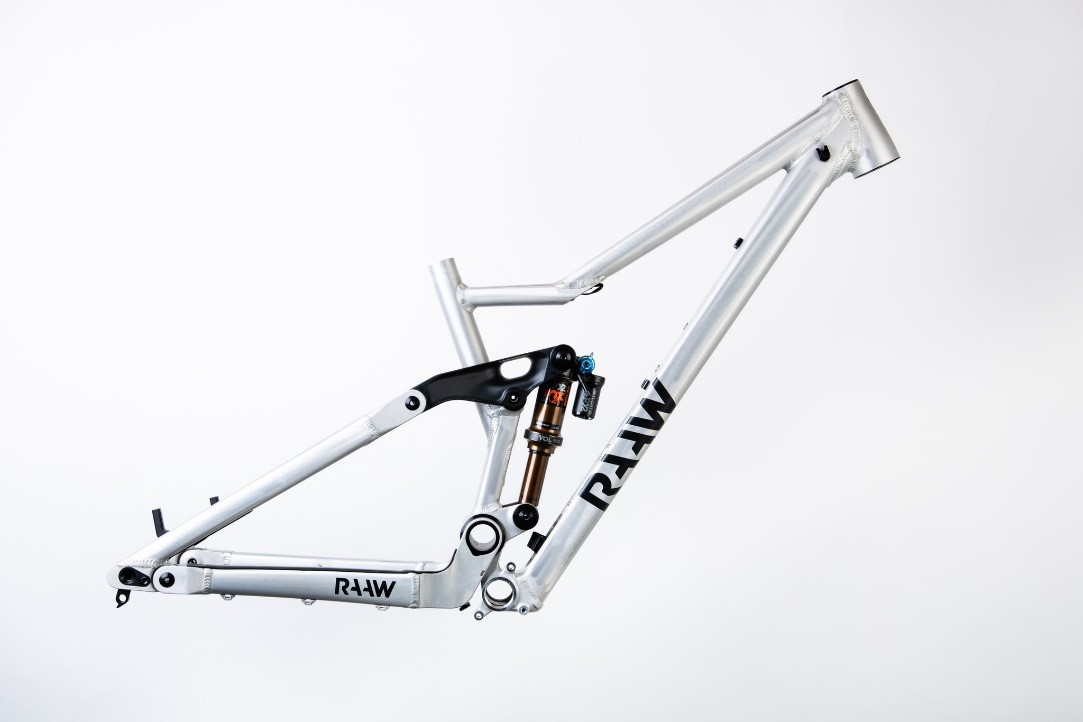
\includegraphics[scale=0.8]{霍斯特鏈懸掛.jpg} 
        %照片須放在和文檔相同之資料夾內
        \caption{霍斯特鏈懸掛} %有caption的圖才會編入目錄中
        \label{fig:scale} %此處的label相當於一個圖片的專屬標誌,目的是方便上下文的引用
    \end{figure}
     \begin{figure}[hbt!]
        \centering
        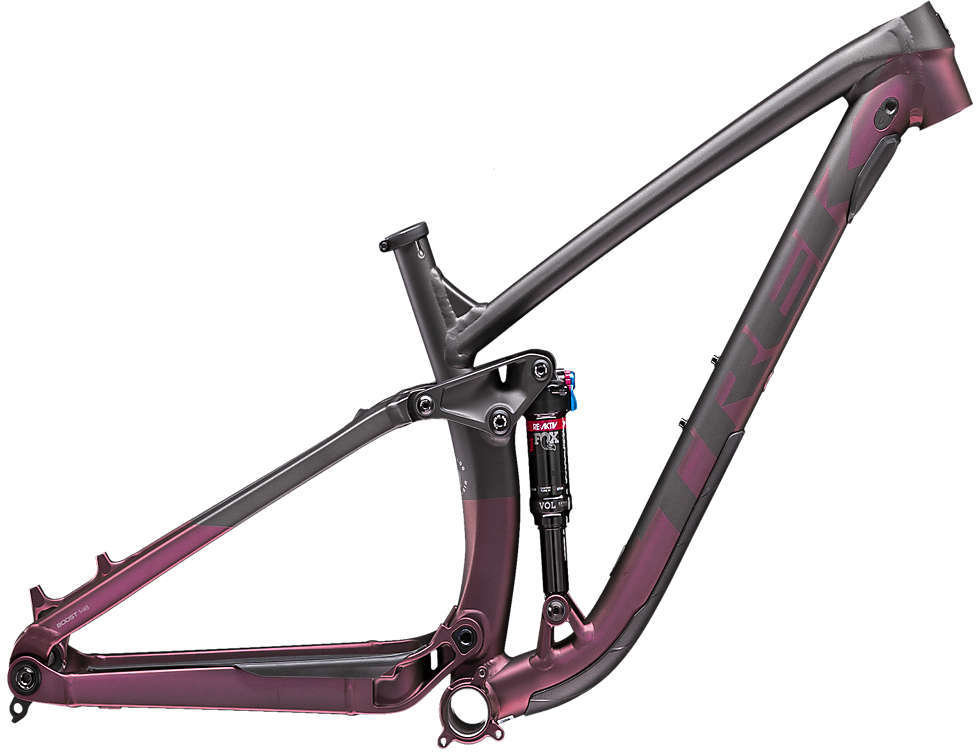
\includegraphics[scale=0.2]{霍斯特鏈懸掛2.jpg} 
        %照片須放在和文檔相同之資料夾內
        \caption{霍斯特鏈懸掛} %有caption的圖才會編入目錄中
        \label{fig:scale} %此處的label相當於一個圖片的專屬標誌,目的是方便上下文的引用
    \end{figure} 
        \chapter{Pyslvs-UI 套件介紹}
      \section{Pyslvs-UI 架構與原理}
      \fourteen {Pyslvs-UI是一套利用Python3與PyQt5建立的平面機構模擬與合成系統。機構模擬與合成的主要核心包括Python-Solvespace幾何約束求解程式庫、三角幾何函式程式庫(tinycadlib)、演算程式庫(ADesign)、幾何約束求解程式庫(bgfs)、類型合成程式庫(topologic)、數目合成程式庫(number)等。其中,ADesign演算程式庫內包含Real-coded Genetic Algorithm (RGA)、Differential Evolution(DE)與Firefly Algorithm (Firefly)等三種,用於平面機構尺寸合成演算}
      \subsection{平面連桿機構模擬}
      \item Python的Solvespace:Solvespace的核心是與Cython綁定在一起。
      \item Pyslvs:使用Cython解決SketchSolve的核心,其中包括平面機構的創新設計方法。
      \fourteen {SketchSolve是一個可用於解決CAD軟件中發現的幾何約束問題的項目。
Cython是針對python編程語言和擴展的Cython編程語言(基於Pyrex)的優化靜態編譯器。}
      \subsection{機構合成}
      \fourteen {進行機構設計與合成主要流程分為尺寸合成、數目合成、構造合成與運動學模擬,而運動學模擬則是進行分析前面的合成項目。 }
      \bf{尺寸合成:}\hspace*{\fill} \\ 
      \fourteen{通過隨機變量生成具有路徑限制的機構,生成結構參數來自變數設定,也有其它算法選擇,程式內共包含三種算法:實數編碼遺傳算法、螢火蟲算法與差分進化演算法。\hspace*{\fill} \\ 
\item 實數編碼遺傳算法:\fourteen{在遺傳演算法的演算過程中,將設計變數以實數數值表示,稱為實數編碼遺傳演算法(RGA),其演算流程如圖3.3(1)。}\hspace*{\fill} \\ 
\item 螢火蟲算法:\fourteen{其演算法是模擬螢火蟲離散的閃爍行為,算法將計算群體中螢火蟲的相對亮度和吸引度,並根據相對亮度決定螢火蟲的移動方向;更新螢火蟲的空間位置,對處在最佳位置的螢火蟲進行隨機移動;根據更新後螢火蟲位置,重新計算螢火蟲的亮度,最終輸出群體極值點和最優個體數值,演算流程如圖3.3(2)。}\hspace*{\fill} \\ 
\item 差分進化演算法:\fourteen{是一種求解最佳化問題的進化演算法,其算法]]]原理採用對個體進行方向擾動,以達到對個體的函式值進行下降的目的,同其他進化演算法一樣,差分進化演算法不利用函式的梯度資訊,因此對函式的可導性甚至連續性沒有要求,適用性很強,演算流程如圖3.3(3)。}\hspace*{\fill} \\ 
}
      \bf {數目合成:}
      \bf {構造合成:}
      \subsection{圖形化使用介面}
      \fourteen{Qt是一個C++應用程式跨平台開發框架,被廣泛應用於開發圖形化介面程式。主要特色為以Qt開發的程式軟體,不須修改原始碼,使用相同的程式碼皆可在支援的平台上執行與編譯,自動依照平台的差異,展示該平台自有的圖形介面風格}
      \section{Pyslvs-UI 編譯}
      \section{Pyslvs-UI 範例}
        \chapter{登山車避震機構}
      \section{避震機構合成}
      \fourteen {機構合成設計需求為騎乘姿勢改變時或遇到顛頗不整的路時仍能保持整體的平衡,即Anti-squat及Anti-rise的數值能在100%附近,而上述合成需求之適應函數可表示為}
      \section{避震機構評量}
      \subsection{Anti-squat}
      \fourteen {當加速時因不同騎乘姿勢導致的重心位置變化而產生的力量轉移會讓懸架受壓縮力,而Anti-squat即為抵抗此後沉的能力。}
       \begin{itemize}
       \item > 100\%: 表示足以抵抗後沉的力量,而超過的力量將會變成拉伸力
       \item 100\%: 表示完全平衡了負載,即懸吊沒受到壓縮力或拉伸力
       \item 0~100\%: 表示部分後沉力量被抵抗
       \item < 0\%: 表示所有的後沉力量皆無被抵抗
       \end{itemize}
       \hspace*{\fill} \\
       \subsection{Anti-rise}
       \fourteen {在剎車的時候因為力量轉移的關係導致後輪產生升起的情況,而Anti-rise即為抵抗此後升現象的能力。}
       \begin{itemize}
       \item > 100\%: 表示足以抵抗後升的力量,而超過的力量將會變成壓縮力
       \item 100\%: 表示完全抵抗了剎車產生的後升現象
       \item 0~100\%: 表示部分後升力量被抵抗
       \item < 0\%: 表示所有的後升力量皆無被抵抗
       \end{itemize}
       \hspace*{\fill} \\
       \subsection{Leverage Ratio}
       \fourteen {Leverage ratio是避震器壓縮量和後輪行程的比值,當較大的槓桿比率會對避震器產生較大的衝擊,而在騎乘時對於地形變化的感受度較不敏感,相反地較小的槓桿比率對於地形的敏感度較高。}
       \hspace*{\fill} \\
      \section{避震機構分析範例}
    
        \chapter{結論}
        {\begin{flushleft}
        \sixteen {內文內文內文123ABC}
        \end{flushleft}

        \chapter{未來研究建議}
        {\begin{flushleft}
        \sixteen {本專題以已建立一流程從尺寸合成至動態模擬軟體進行運動模擬,後續可將運動系統改為動力系統並利用有限元素法對該避震機構進行受力情況的分析。}
        \begin{figure}[hbt!]
        \centering
        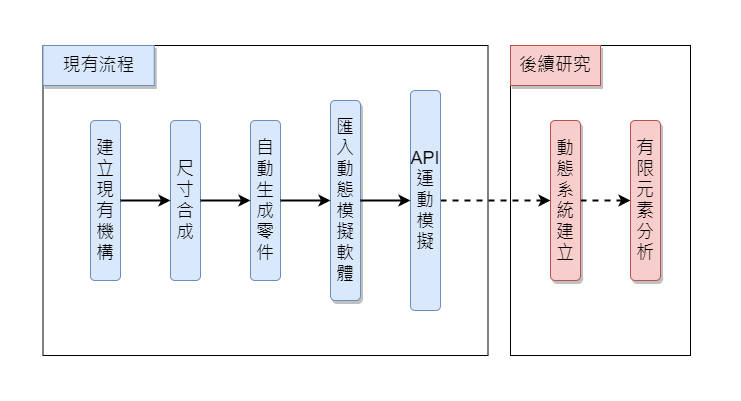
\includegraphics[scale=0.6]{follow-up research.png}
        \caption{後續研究}
        \label{fig:scale}
    	\end{figure}
        \end{flushleft}
        \newpage
        \addcontentsline{toc}{chapter}{\fourteen{參考文獻}}
	\begin{center}
	\twenty \bf{參考文獻}\\
	\end{center}
	\begin{flushleft}
	\fourteen
	{生產自動化是現今工業界中最重要的一環,如何以更低的成本與縮短生產製程,		來提高在國際上的競爭力,是大家所努力的目標,而身為未來二十一世紀的一員,		更需了解其重要性。}
    \end{flushleft}
    \newpage
    
    \addcontentsline{toc}{chapter}{\fourteen{誌謝}}
    \begin{center}
	\twenty \bf{誌謝}\\
	\end{center}
	\begin{flushleft}
	\fourteen
	{生產自動化是現今工業界中最重要的一環,如何以更低的成本與縮短生產製程,		來提高在國際上的競爭力,是大家所努力的目標,而身為未來二十一世紀的一員,		更需了解其重要性。}
    \end{flushleft}
    \newpage
    
    \addcontentsline{toc}{chapter}{\fourteen{作者簡介}}
    \begin{center}
	\twenty \bf{作者簡介}\\
	\end{center}
	\begin{flushleft}
	\fourteen
	{生產自動化是現今工業界中最重要的一環,如何以更低的成本與縮短生產製程,		來提高在國際上的競爭力,是大家所努力的目標,而身為未來二十一世紀的一員,		更需了解其重要性。}
    \end{flushleft}
\end{document} 